\documentclass[runningheads]{llncs}
\usepackage[T1]{fontenc}
\usepackage{graphicx}
\usepackage{amsmath,amssymb}
\usepackage{booktabs}
\usepackage{algorithm}
\usepackage{algpseudocode}
\usepackage[hidelinks]{hyperref}

\begin{document}

% Replace with your title; \titlerunning is the short form printed in the page header.
\title{Detecting Schema Drift in Streaming Data Pipelines with Mergeable Sketches}
\titlerunning{Detecting Schema Drift in Streaming Data Pipelines}

% Authors and their institutes. \inst{n} links an author to institute n.
\author{Lukas Brandt\inst{1} \and
Aisha Rahman\inst{1,2} \and
Tom\'as Herrera\inst{2}}
\authorrunning{L. Brandt et al.}

\institute{Institute for Data Systems, Lindenau University, Leipzig, Germany\\
\email{\{lukas.brandt,aisha.rahman\}@lindenau.example}
\and
Streamline Analytics GmbH, Berlin, Germany\\
\email{tomas.herrera@streamline.example}}

\maketitle

% Replace with your abstract (150 to 250 words).
\begin{abstract}
Streaming pipelines break when the structure of incoming records changes without notice: a field is renamed, a number arrives as text, or an optional field stops appearing. Such schema drift is usually found hours later, when a downstream report is wrong. We describe a detector that summarizes the structure of each stream partition in a small mergeable sketch and compares sketches across time windows. The sketch needs 2.4 kB per partition, can be merged in any order, and bounds the probability of missing a change that affects at least a fraction $\varepsilon$ of records. On three production pipelines with 10 million events per hour, the detector reported 46 of 48 injected changes within one second and raised two false alarms in a week, while adding 1.8\% to processing time.

\keywords{Data streams \and Schema evolution \and Sketches \and Data quality.}
\end{abstract}

\section{Introduction}\label{sec:introduction}
A streaming pipeline reads records from a log, transforms them and writes the results to tables, dashboards and other services. Systems such as Kafka~\cite{kreps2011kafka} and Spark~\cite{zaharia2012resilient} made these pipelines routine, and one team's output is now commonly another team's input. The record structure, or \emph{schema}, is the contract between them, and it is rarely enforced.

When a producer changes its records, consumers often keep running. A renamed field is read as missing, a missing value becomes zero, and the totals on a dashboard quietly drop. We call an unannounced change of this kind \emph{schema drift}. It differs from concept drift~\cite{gama2014survey}, in which the structure stays the same and the distribution of values changes.

Checking every record against a declared schema catches drift immediately, but it requires a schema to exist and to be kept up to date, and it stops the pipeline for changes that are harmless. We take a different approach: observe the structure that records actually have, summarize it compactly, and report when the summary changes.

The paper makes three contributions:
\begin{enumerate}
  \item a sketch of record structure that is small and mergeable, so it fits the parallel execution model of stream processors (Sect.~\ref{sec:method});
  \item a bound on the probability that a change goes unnoticed (Theorem~\ref{thm:bound});
  \item an evaluation on three production pipelines (Sect.~\ref{sec:evaluation}).
\end{enumerate}

\section{Background and Related Work}\label{sec:background}
\subsection{Stream Processing}
Stream processors divide a stream into partitions that are handled in parallel and combine partial results afterwards, an idea that goes back to MapReduce~\cite{dean2008mapreduce}. The Dataflow model~\cite{akidau2015dataflow} adds windows, which group records by the time they were produced. Any summary we compute must therefore be mergeable: combining the summaries of two partitions has to give the summary of their union.

\subsection{Schemas and Their Evolution}
Schema registries store a declared schema per stream and reject records that do not match. They work well when every producer uses them. In the pipelines we studied, between 20\% and 35\% of streams had no registered schema, mostly because they were produced by third-party systems.

\begin{definition}[Structural signature]\label{def:signature}
The \emph{structural signature} of a record is the set of pairs $(p, t)$, where $p$ is the path of a field in the record and $t$ is the type of its value. Two records have the same structure if their signatures are equal.
\end{definition}

For example, the record \texttt{\{"id": 7, "tags": ["a"]\}} has the signature $\{(\mathit{id}, \mathit{int}), (\mathit{tags}, \mathit{array}), (\mathit{tags}[\,], \mathit{string})\}$. Drift, in these terms, is a change in how often each pair occurs.

\section{Method}\label{sec:method}
Fig.~\ref{fig:pipeline} gives an overview. Each partition maintains a sketch of the signatures it has seen in the current window. At the end of the window the sketches are merged and compared with the merged sketch of the previous window.

\begin{figure}[t]
  \centering
  % Replace with your own figure: upload an image and change the file name below.
  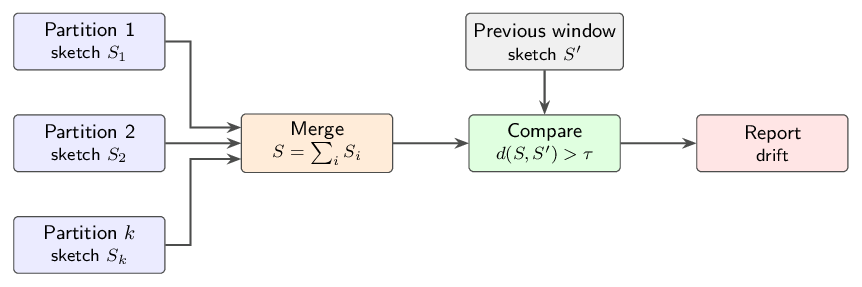
\includegraphics[width=0.95\textwidth]{figures/pipeline.png}
  \caption{Stages of the detector. Sketches are built per partition, merged per window, and compared with the previous window; a difference above the threshold raises a report.}
  \label{fig:pipeline}
\end{figure}

\subsection{The Sketch}
The sketch is an array $S$ of $m$ counters. For every pair $(p, t)$ in a record's signature we increment $S[h(p, t)]$, where $h$ maps pairs to $\{1, \dots, m\}$ uniformly. We also count the number of records $n$. Two sketches with the same $m$ and $h$ are merged by adding their arrays and their record counts, which is associative and commutative.

\subsection{Comparing Windows}
Let $S$ and $S'$ be the sketches of two consecutive windows with $n$ and $n'$ records. We compare the relative frequencies of the counters,
\begin{equation}\label{eq:distance}
  d(S, S') = \max_{1 \le j \le m} \left| \frac{S[j]}{n} - \frac{S'[j]}{n'} \right| ,
\end{equation}
and report drift when $d(S, S') > \tau$ for a threshold $\tau$. Algorithm~\ref{alg:detect} summarizes the procedure.

\begin{algorithm}[t]
\caption{Drift detection for one window}
\label{alg:detect}
\begin{algorithmic}[1]
\Require records $R_1, \dots, R_k$ of the $k$ partitions; previous sketch $S'$ with count $n'$; threshold $\tau$
\Ensure \textsc{true} if drift is detected
\For{$i \gets 1$ \textbf{to} $k$} \Comment{in parallel}
  \State $S_i \gets \mathbf{0}$; $n_i \gets 0$
  \ForAll{records $r \in R_i$}
    \ForAll{$(p, t) \in \Call{Signature}{r}$}
      \State $S_i[h(p, t)] \gets S_i[h(p, t)] + 1$
    \EndFor
    \State $n_i \gets n_i + 1$
  \EndFor
\EndFor
\State $S \gets \sum_i S_i$; $n \gets \sum_i n_i$ \Comment{merge}
\State \Return $d(S, S') > \tau$
\end{algorithmic}
\end{algorithm}

\subsection{Guarantee}
A change is \emph{$\varepsilon$-significant} if it alters the presence or type of some field in at least a fraction $\varepsilon$ of the records of a window.

\begin{theorem}\label{thm:bound}
Let $\tau = \varepsilon / 2$ and let both windows contain at least $n$ records. An $\varepsilon$-significant change is reported with probability at least $1 - 2\exp(-n \varepsilon^2 / 8) - 1/m$.
\end{theorem}

\begin{proof}[Sketch]
The changed pair occupies some counter $j$. With probability at least $1 - 1/m$ no pair with an opposite change of the same size shares that counter, so the expected relative frequencies of counter $j$ differ by at least $\varepsilon$. By Hoeffding's inequality each observed frequency lies within $\varepsilon / 4$ of its expectation with probability at least $1 - \exp(-n \varepsilon^2 / 8)$, and a union bound over the two windows gives the claim. \qed
\end{proof}

With $m = 1200$ counters of two bytes each, the sketch occupies 2.4~kB, and for $n = 10^5$ and $\varepsilon = 0.02$ the bound exceeds 0.98.

\section{Evaluation}\label{sec:evaluation}
\subsection{Setup}
We ran the detector for one week on three pipelines operated by an analytics company: order events (P1), application logs (P2) and sensor telemetry (P3). Windows were one minute long. To measure detection we injected 48 changes of four kinds into copies of the streams, each affecting between 2\% and 100\% of records. As a baseline we compared complete signatures between windows, which is exact but must ship every distinct signature to the coordinator.

\subsection{Results}
Table~\ref{tab:results} lists the outcome per pipeline. The detector found 46 of the 48 injected changes; the two it missed affected 2\% of records in P2, the pipeline with the most varied structure. It raised two false alarms in the week, both during a deployment that briefly doubled the share of one record type.

\begin{table}[t]
  \caption{Detection results for one week per pipeline. Overhead is the increase in processing time compared with the pipeline without the detector.}
  \label{tab:results}
  \centering
  \begin{tabular}{lrrrrr}
    \toprule
    Pipeline & Events/h & Injected & Detected & False alarms & Overhead \\
    \midrule
    P1 Orders    &  3.1 M & 16 & 16 & 0 & 1.2\% \\
    P2 Logs      & 10.4 M & 16 & 14 & 2 & 2.6\% \\
    P3 Telemetry &  6.7 M & 16 & 16 & 0 & 1.7\% \\
    \midrule
    Total        & 20.2 M & 48 & 46 & 2 & 1.8\% \\
    \bottomrule
  \end{tabular}
\end{table}

Fig.~\ref{fig:delay} shows how quickly a change is reported as the stream grows. Because sketches are merged rather than recomputed, the delay of our detector falls below one second after three million events, whereas the full comparison stays above one second throughout.

\begin{figure}[t]
  \centering
  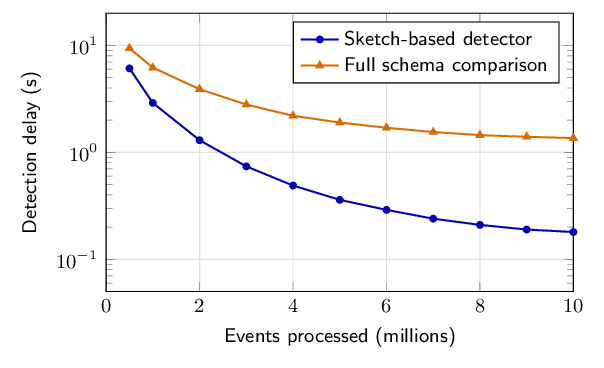
\includegraphics[width=0.8\textwidth]{figures/detection-delay.png}
  \caption{Time from an injected change to its report, as a function of the number of events processed.}
  \label{fig:delay}
\end{figure}

\subsection{Discussion}
The sketch does not say which field changed, only that the structure did. In practice the report includes the five counters with the largest difference, and an engineer resolved the field from them in under a minute in all but one case. Changes confined to rare record types remain hard to detect with any fixed threshold.

\section{Conclusion}\label{sec:conclusion}
Schema drift can be detected without a declared schema by summarizing the structure of records in a mergeable sketch and comparing consecutive windows. The sketch is small, fits the parallel execution model of stream processors, and comes with a bound on missed changes. In a week on three production pipelines it found 46 of 48 injected changes with two false alarms and 1.8\% overhead. Future work includes identifying the changed field directly and adapting the threshold to the variability of each stream.


% Thank people and funders here, or delete the block.
\subsubsection*{Acknowledgements}
We thank the platform team at Streamline Analytics for access to their pipelines. This work was funded by the Saxon Digital Research Fund (grant SDR-2025-08).

\bibliographystyle{splncs04}
\bibliography{references}

\end{document}
